% add option draft to skip images
\documentclass[12pt,a4paper,twosided,open=right]{scrbook}
% \documentclass[12pt,a4paper,twosided,open=right,draft]{scrbook}

% Entwickelt auf Basis von Carsten Kerns Template.

\usepackage[backend=biber,style=alphabetic,maxalphanames=60,maxbibnames=10]{biblatex}
% \usepackage[backend=bibtex,style=alphabetic]{biblatex}
% \usepackage{natbib}
\usepackage[ngerman]{babel}
\usepackage[utf8]{inputenc}
\usepackage{csquotes}
\usepackage{ifthen}
\usepackage{xargs}
\usepackage{amsmath}
\usepackage{amsfonts}
\usepackage{amssymb}
\usepackage{graphicx}
\usepackage{svg}
% \usepackage{fancyhdr}
\usepackage{tabularx}
\usepackage{geometry}
\usepackage{setspace}
\usepackage[right]{eurosym}
\usepackage[printonlyused]{acronym}
\usepackage{subfig}
\usepackage{floatflt}
%\usepackage{color}
\usepackage{xcolor}
\usepackage{colortbl}
\usepackage{paralist}
\usepackage{array}
\usepackage{multirow}
% \usepackage{titlesec}
\usepackage{parskip}
% \usepackage[subfigure,titles]{tocloft}
\usepackage[pdfpagelabels=true,colorlinks=true,linkcolor=black,anchorcolor=black,citecolor=black,filecolor=black,menucolor=black,runcolor=black,urlcolor=black]{hyperref}
\usepackage{booktabs}
\usepackage[lighttt]{lmodern}
\usepackage{mathabx}

\usepackage{listings}
\lstset{basicstyle=\footnotesize, captionpos=b, breaklines=true, showstringspaces=false, tabsize=2, frame=lines, numbers=left, numberstyle=\tiny, xleftmargin=2em, framexleftmargin=2em}

\geometry{a4paper, top=27mm, left=25mm, right=15mm, bottom=27mm, headsep=10mm, footskip=12mm}

% make lstinline be normalsize but keep displayed listings small
\makeatletter
\lstdefinestyle{mystyle}{
  basicstyle=%
    \ttfamily
    \lst@ifdisplaystyle\scriptsize\fi
}
\makeatother

\lstset{
	language=C++,
	% basicstyle=\ttfamily\scriptsize,
	style = mystyle,
	% basicstyle=\ttfamily\scriptsize,
	keywordstyle=\bfseries\ttfamily,
	% commentstyle=\color{LimeGreen}\ttfamily,
	commentstyle=\color{gray}\ttfamily,
	emphstyle={\color{Purple!90!black}},
	tabsize=4,
	morekeywords={nullptr,nullptr_t,vector,string,std,list,map,pair,set,size_t,endl,cout,move},
	emph={},
	showstringspaces=false,
}

\setcapindent{0pt}
\setkomafont{captionlabel}{\bfseries}

\DefineBibliographyStrings{ngerman}{
	andothers = {{et\,al\adddot}},
}


\DeclareLabelalphaTemplate{
  \labelelement{
    \field[final]{shorthand}
    \field{label}
    \field[strwidth=3,strside=left,ifnames=1,names=1]{labelname}
    \field[strwidth=1,strside=left,names=1-3]{labelname}
  }
  \labelelement{
    \field[strwidth=2,strside=right]{year}
  }
}
\renewcommand*\labelalphaothers{$^\Asterisk\mkern-.8mu$}

\newcommandx{\student}[3][]{
	\def\studentName{#1}%
	\def\studentMatnr{#2}%
	\def\studentStudiengang{#3}%
}

\newcommandx{\MyTitelseite}[8][]{
\thispagestyle{empty}
\ifthenelse{\equal{#1}{}}{
	
\includegraphics[scale=0.2]{lib/oth-logo.png}
}{
	
\includegraphics[scale=0.2]{lib/oth-logo.png}\hfill\includegraphics[scale=0.5]{#1}
}
\begin{center}
\ifthenelse{\equal{#2}{2}}{ % then
	\vspace*{2cm}
	\Large
	\textbf{Ostbayerische Technische Hochschule Regensburg}\\
	\textbf{Fakultät für Informatik und Mathematik}\\
	\vspace*{2cm}
	\Huge
	\textbf{#3}\\[1em]
	\large
	Zur Erlangung des akademischen Grades des\\
	\ifthenelse{\equal{#3}{Bachelorarbeit}}{Bachelor of Science (B.Sc.)}{Master of Science (M.Sc.)}\\
	\vspace*{1cm}
	\Large
	\textbf{#4}\\
}{ % else
	\vspace*{1cm}
	\Large
	\textbf{#4}\\
	\vspace*{2cm}
	\large
	An der Fakultät für Informatik und Mathematik der\\
	Ostbayerischen Technischen Hochschule Regensburg\\
	im Studiengang\\[2em]
	\textbf{\studentStudiengang}\\[2em]
	eingereichte\\
	\vspace*{1cm}
	\Large
	\textbf{#3}\\[2em]
	\large
	zur Erlangung des akademischen Grades des\\
	\ifthenelse{\equal{#3}{Bachelorarbeit}}{Bachelor of Science (B.Sc.)}{Master of Science (M.Sc.)}
	\vspace*{1cm}
	\Large
}
	\vfill
	\normalsize
	%\newcolumntype{x}[1]{>{\raggedleft\arraybackslash\hspace{0pt}}p{#1}}
	\begin{tabular}{rl}%{6cm}p{7.5cm}}
	    \rule{0mm}{1ex}\textbf{Vorgelegt von:} & \studentName \\
		\rule{0mm}{1ex}\textbf{Matrikelnummer:} & \hspace*{-0.5em}\begin{tabular}[t]{r}\studentMatnr\end{tabular} \\ 
		\ifthenelse{\equal{#2}{1}}{~\\}{\rule{0mm}{1ex}\textbf{Studiengang:} & \studentStudiengang \\[2em]}
		\rule{0mm}{1ex}\textbf{Erstgutachter:} & #5 \\ 
		\rule{0mm}{1ex}\textbf{Zweitgutachter:} & #6 \\[2em]
		\rule{0mm}{1ex}\textbf{Abgabedatum:} & #7 \\ 
	\end{tabular} 
\end{center}
\pagebreak
}



% ein paar nützliche Kommandos

\newcommand\defsec[1]{\label{sec:#1}}
\newcommand\refsec[1]{\ref{sec:#1}}

%\newcommand\todo[1]{\textcolor{red}{[{\textbf{TODO}} #1]}}
\newcommand\todo[1]{} % remove todos

%\newcommand\new[1]{\textcolor{new}{{#1}}}
\newcommand\new[1]{#1} % plain text
%\newcommand\old[1]{\textcolor{gray}{{\sout{#1}}}}
\newcommand\old[1]{} % remove old stuff

\definecolor{lgdv}{rgb}{.80,.23,.13}
\definecolor{agreen}{rgb}{.2,.8,.2}
\definecolor{jorange}{rgb}{.9,.6,.0}
\definecolor{new}{rgb}{.8,.4,.4}

\newcommand\NOTE[3]{\textcolor{#1}{[#2: #3]}}
\newcommand{\TODO}[1]{\\ \colorbox{yellow}{TODO: #1}\\}

%\newcommand\kai[1]{\NOTE{lgdv}{Kai}{#1}}
\newcommand\kai[1]{} % remove notes
%\newcommand\niko[1]{\NOTE{jorange}{Niko}{#1}}
\newcommand\niko[1]{} % remove notes

\newcommand\To{\ensuremath{\to}}
\newcommand\hi[1]{\textcolor{red}{#1}}

\let\shortcite=\cite

\addbibresource{bib.bib}

\begin{document}

% ----------------------------------------------------------------------------------------------------------
% Titelseite
% ----------------------------------------------------------------------------------------------------------
\newcommand{\stud}{Emanuel Erben}  % Ihr Name
\student{\stud}
{3174817}						% Matrikelnummer
{Informatik}					% Studiengang

\MyTitelseite{}					% Optionales Logo des extern betreuenden Unternehmens
% \MyTitelseite{pics/mathcomm}	% Optionales Logo des extern betreuenden Unternehmens
{1}								% Style der Titelseite (1 oder 2)
{Bachelorarbeit}				% Typ der Abschlussarbeit (\in {Bachelorarbeit, Masterarbeit})
{Vergleich verschiedener Ansätze der Multiplattform Applikationsentwicklung anhand einer Beispiel-Anwendung}				% Thema der Arbeit						
{Prof.\ Dr.-Ing.\ Kai Selgrad}		% Betreuer
{Prof.\ Dr.\ Name des Zweitgutachters}	% Zweitgutachter
{15.09.\the\year}				% Abgabedatum

\thispagestyle{empty}
~\pagebreak

\setcounter{page}{1} 

Das muss an den Kapiteln noch gemacht werden:

0.Abstract:
Ende nochmal umschreiben
1.Motivation:
Einordnung nochmal anschauen und insgesamt überarbeiten.
Die Arbeitsbeschreibung

Related:
Überarbeiten und eventuell Performance Untersuchung mit neuem Austauschen.

3.Grundlagen:
Projektbeschreibung : 
noch machen
Themenabgrenzung :
Mal schauen ob noch mehr und bei Spiel Ende nochmal nachschauen.
Erklärung warum nur Smartphone Applikationen betrachtet.
Begriffe:
umstellen
Arten:
Nativ und Hybrid soweit an Selgrad, Rest muss überareiten
drüberlesen

4. Einleitung
Vielleicht nochmal bisl spannender
4.1 Nativ

4.2 hybrid

4.3 Flutter
ausmisten
ordentlich neu schreiben

4.4 hybrid flutter

5.Auswertung
Noch komplett
kriterien aussuchen
Werte zusammenschreiben, messen oder nachforschen
Tabellen und sonstiges erstellen

6.Fazit
Noch komplett


% ----------------------------------------------------------------------------------------------------------
% Abstract
% ----------------------------------------------------------------------------------------------------------
% \thispagestyle{empty}
\setstretch{1.15} % Zeilenspacing
\chapter*{Abstract}

\bigskip 

In den letzten Jahren nutzen immer mehr Leute nicht mehr nur noch Computer sondern vor allem auch ihre Smartphones, um auf die verschiedenen Plattformen, Konten und Online-Anwendungen zuzugreifen. Um eine Anwendung auf den verschiedenen Mobilen-Plattformen veröffentlichen zu können haben Entwickler daher oft nur die Möglichkeit eine App für jeden einzelne Plattform zu schreiben oder eine Website zu bauen. In den letzten Jahren hat sich jedoch hier eine dritte Möglichkeit augetan. Hier wird versucht mit einer einzigen Programmierung eine Applikation für möglichst viele Plattformen zu erzeugen. So genannte Cross-Plattform-Applikationen

In dieser Arbeit soll anhand einer bestehenden Website verschiedene Applikationen programmiert werden und dabei verschiedene Entwicklungsanätze und ihre Vor und Nachteile beleuchtet werden. Dabei wird vor allem die Android Plattform und die Programmiersprachen Kotlin bnzw. Dart beleuchtet werden. Dazu werden verschiedene Android und Flutter Applikationen vorgestellt und anhand ausgewählter Kriterien bewertet werden. 
\TODO{Ende muss noch umgeschrieben werden}
Am Ende soll ein Fazit gezogen werden, bei dem vor allem darauf eingegangen werden soll, welche Probleme, bzw. Herausforderungen bestehen und was ein guter Weg wäre um Applikationen zu entwickeln.


\frontmatter

% ----------------------------------------------------------------------------------------------------------
% Inhaltsverzeichnis
% ----------------------------------------------------------------------------------------------------------
\tableofcontents
\vfill
\pagebreak

% % ----------------------------------------------------------------------------------------------------------
% % Abbildungsverzeichnis
% % ----------------------------------------------------------------------------------------------------------
% \listoffigures
% \vfill
% \pagebreak
% 
% % ----------------------------------------------------------------------------------------------------------
% % Tabellenverzeichnis (optional)
% % ----------------------------------------------------------------------------------------------------------
% \listoftables
% \vfill
% \pagebreak

% ----------------------------------------------------------------------------------------------------------
% Listingsverzeichnis (optional; Code nur, wenn wirklich sinnvoll und wichtig)
% ----------------------------------------------------------------------------------------------------------
\lstlistoflistings
\vfill
\pagebreak


% ----------------------------------------------------------------------------------------------------------
% Inhalt
% ----------------------------------------------------------------------------------------------------------
\setstretch{1.15}


\mainmatter


\chapter{Motivation}




Die Entwicklung im Bereich der mobilen Anwendungsentwicklung ist in den letzten Jahren sehr hoch. Nicht nur das immer mehr Technologien und Frameworks in Richtung Hybride Appentwicklung entwickelt werden. Es werden auch immer mehr Erweiterungen für bestehende Technologien geschrieben, die eine möglichst effiziente mobile App ermöglichen sollen. Aber auch die nativen Apps ändern sich stetig und die dahinter stehenden Programmiersprachen bekommen stetig neue Änderungen und werden weiterentwickelt.

Wenn man nun eine eigene Applikation schreiben will, steht man erstmal vor der Frage wie und wo man anfängt.
Fragen nach der richtigen Programmiersprache bzw. dem richtigen Framework kommen dann auf.

Langezeit gab es hier sehr konkrete Antworten. Da die meisten leute vlt. nur einen Heimcomputer besaßen, entwickelte man meist nur Computeranwendungen oder eben Webapplikationen, die jeder von überall aus aufrufen konnte, ohne die Applikation auf seinem eigenen Computer installieren zu müssen.

Mit der Ära der Smartphones jedoch änderte sich das etwas, denn auch hier kann man natürlich Webapplikationen nutzen, jedoch sind diese oft nicht angepasst gewesen.

Daraus entstand eine Zeit wo mobile Applikationen speziell für das eigene Smartphone entwickelt wurden. Es gab auch einige neue Ansätze und Funktionalitäten, die man so nutzen konnte, die davor nicht nutzbar waren. Hier wurden oft Applikationen mit Swift, der Programmiersprache für iOS und Java bzw. mittlerweile Kotlin für Android Applikationen. Hier entstanden also sogar eigene Programmiersprachen für die jeweiligen Plattformen zur sogennanten nativen Entwicklung.

Wenn man jedoch nun auf mehreren Plattformen seine Applikationen veröffentlichen wollte, so musste man zwei eigene Applikationen in zwei unterschiedlichen Programmiersprachen schreiben. 

Daraus entstand der Wille dass doch zu vereinigen und sogennante Multi-Plattform-Applikationen oder auch Cross-Plattform-Applikationen zu entwickeln.
Und hier fing das Problem an. Da dies eine frei Entwickelte Sache war, wo zunächst keiner der großen Plattformanbieter dahinter stand, entstanden viele kleine und auch manchmal größere Frameworks die dieses Problem lösen sollte.

In dieser Zeit gab es auch immer wieder Ansätze großer Firmen, ihre Apps in hybride Apps zu ändern, jedoch tauchen auch immer wieder Berichte darüber auf, dass solche Schritte nach einer anfänglichen Testzeit wieder aufgegeben wurden. So hat etwa Airbnb bereits 2016 mit sogenannten React Native versucht ihre Apps auf eine gemeinsame Codebasis zu bauen. Sie haben das auch einige Zeit probiert, haben dann allerdings 2018 eine Reihe von Blog Einträgen veröffentlicht, in der sie erklären, warum sie React Native damals dann aufgegeben haben und dabei erklärt, dass sie sich deshalb weiter darauf konzentrieren würden, die nativen Apps zu verbessern. 
\TODO Hier mehr zu den Gründen schreiben warum aufgegeben

Durch Beispiele wie dieses, waren App-Entwickler lange Zeit skeptisch gegenüber derartigen Lösungen, da dies auch immer mit großen Änderungen und hohen Investments verbunden waren.
Jedoch gab und gibt es mittlerweile immer mehr Ansätze die es scheinbar schaffen diese Hürden zu überwinden.

Durch aber die eben geschilderte Entwicklung und Berichte, ist die Meinung die man hierzu lesen kann immer sehr unterschiedlich und stark von eigenen Erfahrungen abhängig. 
Deswegen soll in dieser Arbeit drei unterschiedliche Ansätze mit beispielhaften Frameworks und Programmiersprachen betrachtet werden um am Ende vlt eine bessere Einschätzung geben zu können, wie eine solche Entscheidung ausfallen könnte und Gründe für und gegen bestimmte Ansätze geben.



\TODO umschreiben
Auch als Appentwickler nehmen durch immer neue Technologien die entwickelt werden und auch erfolgreich teilweise eingesetzt werden, die Anfragen zu, die eine Entwicklung mit Hilfe von Flutter oder ähnlichen Wünschen. Dennoch ist es immer noch ein Verfahren, das weiter untersucht werden muss und noch nicht überall selbst verständlich benutzt unnd entwickelt werden kann.

Daher ist der Fokus dieser Arbeit einmal an einigen konkreten Beispielen zu untersuchen, wie der aktuelle Stand der Technologie hier ist und zu erforschen, welche Einschränkungen die Frameworks besitzen um hier auch eine gewisse Bewertung zu Benutzbarkeit als Applagentur zu untersuchen.

------
Schon genauere Erklärung:
Wenn man die Idee zu einer App hat, gibt es die große Frage, wie man nun anfängt und welche Programmiersprache / Framework man wählt. Hierfür gibt es ganz verschiedene Ansätze.  

Jedoch noch grundlegender ist die Frage nach der Plattform. Es gab lange Zeiten in der Applikationsentwicklung, dass nur eine Webversion veröffentlicht wurde. Mittlerweile nutzen jedoch viele Menschen nur noch ihr Smartphone und wollen dementsprechend auch nur mit mobilen Versionen auskommen. Man kann natürlich auch im Web veröffentlichte Applikationen auf dem Handy nutzen, jedoch gibt es hier zwei Sachen, die dazu führen können, dass man eine eigenständige App entwickelt.
1. Eine auf mobile angepasste UI. - Auch wenn es heutzutage in fast jedem Framework und vor allem in den gängigen UI-Frameworks verschiedene Ansätze gibt, die eine recht nutzerfreundliche Version für mobilgeräte anbieten, oder manchmal auch sogar komplett eigenständige Oberflächen für mobil angezeigt werden, so kann es doch sinvoll sein, nochmal extra angepasste UI in Form einer Applikation nativ für die Geräte zu entwickeln. Dadurch kann man gezielt Oberflächen für die Plattformen bauen und dabei auf Plattform eigene Design Unterstützungen zugreifen. Die eine Bedienung um einiges besser machen.
2. Nutzung von Hardwarefunktionalität. -  Ein noch viel wichtigerer Punkt ist es, Funktionalität die mobile Endgeräte anbieten, zu nutzen, die etwa auf einem PC nicht nutzbar sind. Dazu zählen unter anderem GPS-Nutzung, Kamerafunktionalitäten, Bluetooth-Verbindungen,.... Diese können zwar mnanchmal auch durch einen PC geboten sein, jedoch ist es hier nicht gegeben, während man bei einem Smartphone sicher davon ausgehen kann, dass die Kamera genutzt werden kann. So können einige Geschäftsprozesse der Applikationen vereinfacht oder umgestaltet werden, so dass eine Nutzung der Applikation für den Nutzer einfacher wird, bzw. es können auch neue Funktionalitäten daraus ergeben, die es eventuell davor nicht gab.

Wenn nun die Entscheidung getroffen wurde, dass man eine mobile Applikation entwickeln will, so gibt es nun verschiedene Ansätze bzw. Frameworks, die zur Verfügung stehen. Dabei gibt es viele verschiedene Frameworks die auf den ersten Blick das selbe tun, aber doch recht unterschiedlich sein können und unter gewissen Ummständen sich manche besser eignen als andere. 
Eine der ersten Fragen die dabei im Raum steht. Gibt es bereits eine Webversion der Applikation.
Wenn nicht, so kann es von Anfang an spannend sein, ein Framework zu wählen, dass wie Flutter eine Cross-Plattform-Applikation erzeugt, wo auch eine Webversion mit gehostet werden kann.
Falls es bereits eine Webversion geben, so geht der Weg eher in Richtung von Nativen- bzw. Hybriden Applikationen, da meißt nur noch einzelne Teile der Applikation entwickelt werden müssen. Dies ist jedoch auch kein Grund eine Cross-Plattform-Entwicklung auszuschließen, da dadurch nur ein Code geschrieben werden muss um etwa beide vorherschenden mobilen Plattformen abzudecken: iOS und Android.

'''Hier könnte man so ein Art Diagramm machen mit Fragen und dann Entscheidungswegen. So nach dem Motto finde dein Framework zur entwicklung einer mobilen Applikation.'''




\chapter{Definitionen und Erklärungen}

Bevor genauer in die Arbeit eingestiegenw erden kann, müssen jedoch erstmal die Ausgangsituation dargestellt, ein paar Begriffe geklärt und das Thema etwas abgesteckt werden.

\section{Projektbeschreibung}
Zu Beginn der Arbeit bestand bereits eine Website, die durch einen internen Workshop konzeptioniert und durch ein Pflichtpraktikum implementiert wurde. Die Website wurde mit der Web-Technologie Elixir gebaut, die sowohl Frontend als auch Backend beinhaltet. Hierbei handelt  es sich um eine Plattform, die das Ziel hat, das Verleihen und Leihen innerhalb von Bekanntschaftskreisen zu vereinfachen/ ermöglichen. Hierfür kann jeder Nutzer seine eigenen, verleihbaren Gegenstände auf der Plattform eintragen. Zusätzlich können Nutzer sogenannte Kreise erstellen und zusammen mit Freunden bzw. Familie beittreten. Jeder kann dann die Gegenstände sehen, die in den verschiedenen Kreisen verfügbar sind, in denen er Mitglied ist. Zur Kontaktaufnahme gibt es ein Chatsystem, bei dem sich Leute Nachrichten hin und her schicken können, um den Austausch zu organisieren.

\section{Funktionsumfang der Beispiel Anwendung}
Um mehrere Unterschiedliche Ansätze implementieren zu können, wurde die App, die entwickelt wurde, auf einen bestimmten Funktionsumfang beschränkt. Dieser soll dabei all das enthalten was bei einer typischen Appbenötigt wird. So hat man einfache Informationsseiten, einen Login, eine Authentifizierung, eine gewisse Art von Navigation, eine Listenansicht, eine Art permanente Speicherung von Daten für den Login und eine Kommunikation mit einem Server um Daten zu erhalten, schicken und evtl zu synchronisieren.

In Abbildung \ref{fig:pageflow} Kann man die in Android und Flutter implementierten Abläufe sehen.  

\begin{figure}[ht]
  \centering
  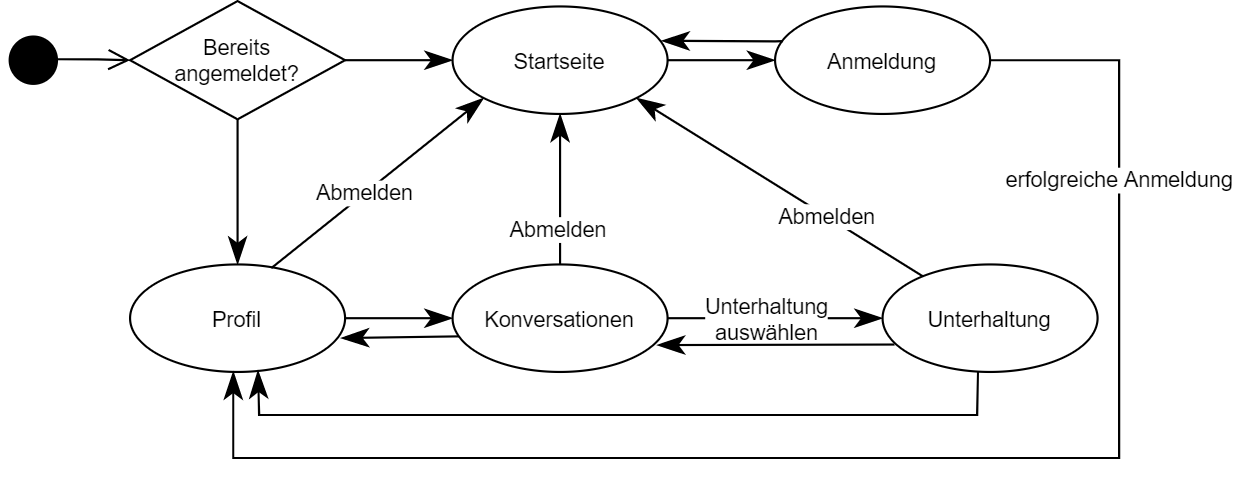
\includegraphics[height=7cm,keepaspectratio]{images/Pageflow_native_flutter.png} 
  \caption{Verbindungen zwischen den Seiten der implementierten Applikation }
  \label{fig:pageflow}
\end{figure}

\section{Themenabgrenzung}
Keine Spiele weil....
Kein iOS weil....


\section{Begriffe}
Wenn in dieser Arbeit von einer App bzw. Applikation geredet wird, so ist hiermit eine Anwendung gemeint, die für mobile Endgeräte, vorallem Smartphones mit den Betriebssystemen Android bzw. iOS gebaut wurden.
Außerdem ist in dieser Arbeit oft die Rede von Multi-Plattform-Anwendungen. Darunter versteht man eine Anwendung, die nicht nur für eine Plattform geschrieben wurde, sondern für mehrere. Das kann etwa die verschiedenen Smartphone Plattformen beinhalten, können aber auch die verschiedenen PC Plattformen mit einbegriffen werden. Eine Anwendung muss dabei auch nicht alle Plattformen beinhalten, sonder kann auch nur zwei Statt Multi-Plattform-Anwendungen wird häufig auch Cross-Plattform-Applikationen als Begriff genutzt, da dies ein in der Industrie häufig benutzter Wortlaut ist. 

\section{Die verschiedenen App Development Framework Klassen}
Wenn man über Applikationsentwicklung für mobile Endgeräte spricht, muss mann zwischen einigen verschiedenen Varianten unterscheiden.
\TODO{Muss auf jeden Fall noch Quellen, noch mehr und umschreiben.}
\subsection{Native Applikationen}
1.Native Apps:
Native Apps sind Applikationen die mit der Plattformspezifischen Programmiersprache für die einzelnen Plattformen entwickeltwerden. Hierbei wird dann in Kotlin für Android oder Swift für iOS sowohl die UI als auch die Logik der App umgesetzt und ist so gesehen ein eigenständiges System, da die dadurch entwickleten Applikationen nur auf der Plattform genutzt werden können, für die sie geschrieben wurden.
Oft verfügen diese Applikationen auch noch über externe Schnitstellen, oder einer Verbindung zu einem Server, um etwa auf Datenhaltung oder andere Dienste zuzugreifen.
Ein Vorteil dieser Art der Entwicklung ist es, dass man sehr gut die verschiedenen Möglichkeiten der jeweiligen Plattform ausnutzen kann. So ist etwa eine Nutzung der Kamera in nativ entwickelten Applikation deutlich einfacher und besser umsetzbar. Dazu kommt, dass man bessere Nutzeroberflächen bauen kann, die auf die mobile Plattform angepasst sind.
Der Nachteil den eine Native Entwicklung jedoch hat ist der Aufwand und die damit verbundenen Kosten. Um für die beiden vorherschenden Plattformen eine Applikation anbieten zu können, braucht man die doppelte Zeit, als wenn man nur eine App entwickelt. Kommt dann noch eine Website und Serveranwendung oder ähnliches hinzu, wird schnell aus einer kleinen Anwendung ein großer Kostenproduzent.
\subsection{Hybride Applikationen}
2. Hybride Apps:
Hybride Apps sind Applikationen die zu gewissen Anteilen aus nativem Code bestehen und zu gewissen Teilen Code, Schnitstellen oder Darstellungen anderer Websiten bzw. Webapplikationen nutzen. Der häufigste Anatz ist es hier, Webappplikationen zu einem gewissen Anteil in einem Frame der Applikation darzustellen und dabei einzelne Seiten durch nativ entwickelte Oberflächen zu ersetzen und die Daten an die Webapplikationen weiter zu geben. 

\subsection{Cross Plattform Applikationen}
3. Cross-Plattform-Apps
Unterscheidung zwischen Webview in App und z.B. Flutter 

\chapter{Entwicklung Nativer Android Application}
Wie bereits erwähnt wird im nativen Bereich lediglich die Android Seite implementiert. Die zugrundeliegenden oft verwendeten Technologien sind in den meisten Fällen auf beiden Seiten vorhanden. Sie haben ihre einzelnen Feinheiten, können aber im Grunde soweit als gleich angesehen werden.

Wenn man eine Android App entwickelt, so muss man wie bei jeder Technologie erstmal ein paar Entscheidungen treffen. Hier gibt es natürlich erstmal die größte Entscheidung der Programmiersprache. Denn selbst wenn man native Applikationen entwickelt so ist dennoch nicht klar definiert bzw. vorgegeben mit welcher Programmiersprache dies geschehen muss. Für iOS sind diese Swift bzw. Objectiv-C. Bei Android gibt es da die Unterscheidung zwischen Java und Kotlin. Diese Entscheidung ist jedoch eher eine kleine. Denn von der Sache her sollte man Kotlin und Swift nutzen, da diese die neuen Sprachen sind die von Google bzw. Apple extra hierfür entwickelt und veröffentlicht wurden. Man kann immer noch die alten Programmiersprachen nutzen und diese sind auch immer noch aktiv in Nutzung und haben viele Forumseinträge und Anleitung für die verschiedensten Problemstellungen. Außerdem bauen die neuen Programmiersprachen grundsätzlich auf den alten auf. So ist Kotlin eine auf Java basierende Programmiersprache die bidirektional übersetzt werden kann. So kann man alten Java Code in die Kotlin App einbinden und automatisch übersetzen lassen. Außerdem wird der Kotlin Code zum bauen der App in Java übersetzt und dann in Java ausgeführt.
Nachdem dies aus dem Weg geschafft ist und wir uns also für Kotlin in diesem Fall entschieden haben, gibt es nun weitere Entscheidungen zu treffen. Bei Android Apps kann man grundsätzlich zwischen zwei verschiedenen Arten des Seitenaufbaus und der Grundarchitektur. 
Diese nennen sich Activitys bzw. Fragments. Sie sind die Entscheidung für eine Art Grundstruktur. Bei Activitys sind die einzelnen Seiten unterschiedliche Klassen und eigenständige Systeme. Jede Activity hat ihren eigenen Context und wird selbständig auf dem Bisldschirm aufgebaut. Danach wird neben ein paar ausnahmen nur zwischen den eigenen Activitys hin und her navigiert um den Ablauf der App nachzubilden.
Bei Fragments haben diese einen geteilten Kontext. Sie werden alle gleichzeitig gebaut und werden dann nur darübergelegt bzw. vom Bildschirm entfernt. Ein großer Vorteil dieser Methode ist, dass man wenn man genügend Platz hat, zwei Bildschirme nebeneinander angezeigt werden können und diese beide normal funktionieren. Bei kleinen Bildschirmen oder unter Umständen kann auch dann nur ein Fragment angezeigt werden. Somit zeigt sich, dass vorallem für Anwendungen die sowohl auf Tablet und Handy Problemlos genutzt werden sollen, Fragments sich gut eignen.
Beide Ansätze haben ihre Vor- und Nachteile.
Für diese Arbeit wurde entschieden auf die Activitys Architektur zurück zu greifen, da sie anfänglich einfacher ist und Schwierigkeiten mit dem Kontextmanagment und dem App Backstack zum navigieren durch die History reibungsloser funktioniert. Außerdem sind Activities aktuell besser dokumentiert und viele Problemlösungen sind für Activities beschrieben.

Nach dem man sich nun für eine Grundarchitektur entschieden hat, müssen ein paar Entscheidungen anhand der Projektarchitektur getroffen werden. Ersteinmal muss man entscheiden ob man eine lokale Offline Datenbank braucht oder ob man eine Onlinedatenhaltung mit eventuell angebundener Serverlogik hat. Natürlich kann auch beides gemacht werden. Jedoch in diesem Fall werden wir nur eine Onlinedatenhaltung benutzen die über eine API angebunden ist. 


Ärgerlich bei der Nativ Entwicklung und Graphql war, dass neu erzeugte Querys erst durch ein Build durchlauf erzeugt wurden, und so etwas längert braucht zur Entwicklung.
\section{Layout}
\section{externe Bibliotheken}
\section{Fazit Nativ}
\chapter{Entwicklung Hybrider Android Application mit WebView}
Es gibt noch einen anderen Weg eine Anwendung auf mehrere Plattforment zu bringen.
Und zwar eine Website in einer nativen App anzuzeigen. So muss man lediglich eine Website schreiben die auch gut auf verschiedenen Bildschirmgrößen angezeigt werden kann. Danach muss man nur noch ein paar Anpassungen an einer nativen Android App vornehmen, um eine Reibungslose funktionalität zu gewährleisten und schon hat man eine Applikation die als Website auf allen Geräten aufgerufen werden kann und man kann sie gleichzeitig noch in eine Webview einbauen, um seinen Nutzern eine Appversion bieten zu können, die diese aus den Appstores herunterladen können.
\section{Abstufungen}
Diese Entwicklung kann jedoch noch generell in zwei unterschiedliche Abstufungen unterteilt werden. 
\section{Reine Webview ohne nativen Anteil}
Hier wird nur die Website auf einem "Canvas" angezeigt und noch ein paar Konfigurationen vorgenommen, damit alle Funktionalität grundsätzlich angeboten werden kann.

\section{Webview gemischt mit Nativer Funktionalität}
Es gibt Optionen einen Nativen anteil in eine WebView App einzubauen.
\subsection{Einbau des Android Adapters in Website um native Funktionalität aufzurufen}
Neben der einfachen WebView kann man wenn die Website Javascript benutzt auch native Funktionalität einbauen. So kann man eine Javascript Verbindung erstellen indem man im Javascript der Website eine Android Adapter aufruft und dort eine Funktion aufruft, die im Android Code definiert ist. So kann man native Funktionalität auf Smartphones nutzen.(Toast beispiel)
\subsection{Mischen zwischen Nativer und Webansicht}
Einen Schritt weiter als davor. Hier schreibt man die Website bereits in einer passenden Technologie/ Sprache, um im Anschluss eine App zu entwickeln, die native und Web Ansichten mischt, um einen möglichst effizienten aber trotzdem nativ aussehenden Look für eine App zu erhalten. Hotwire und Turbo. als Beispiel
Diese Technologie wurde von der Firma Basecamp entwickelt, die schon lange für ihre Plattform eine schnelle Lösung für ihre Websiten gesucht haben. Daher haben sie Hotwire erfunden. Hotwire steht für HTML over Wire. Was das bedeuted ist, dass die Website nicht andauernd komplett neugeladen wird, sondern nur die teile, die auch erneuert werden müssen. Dazu kommt noch einige technologie die das caching und die verarbeitung der benötigten javascript Files handelt und raus kam eine Lösung um schnell und performant Websiten zu laden.
Um das ganze nun auf ein Smartphone zu bringen war die Idee entsanden, dass man hier nicht eine komplette native App schreiben wollte sondern eben eine WebView herzunehmen, in die aber Native Teile gemischt weren, um die Erfahrung der Nutzer möglichst intuitiv zu gestalten. 





\section{Fazit(muss wsl. wo anders hin) zu hybrid}
Auch wenn es auf dem ersten Moment super einfach scheint und es so wirkt, als könnte man so jede Website einfach in eine Applikation stecken, ohne dass man groß wiederholenden Code hat, bzw. dass man mehrmals die komplette Anwendung schreiben muss, sondern ja nur einmal und je nach grad noch einmal Aufwand hineinstecken muss, aber nie in dem Umfang wie für eine komplette native App. 
Es hat auch Nachteile und Gründe, warum dies nicht gern genutzt wird.
Ein aller erster großer Nachteil ist eine reine online Funktionalität. 
\chapter{Entwicklung Cross-Plattform Application mit Flutter}
Notizen zur Entwicklung mit Flutter:


Durch voreinstellung und Erstellen eines Basic screen schon nach wenigen Minuten eine erste laufende "Version" zu sehen.

Hot Reload zeigt sofort sichtbare Änderungen, so dass man gut UI debuggen umbauen und anpassen kann.

Schwer herauszufinden welche Elemente es gibt, wie man sachen konfigurieren kann. Am Anfang nicht sehr intuitiv. Man muss sich auf jeden Fall gut in die Doku einlesen und vlt. auch ein kleines Tutorial machen, bzw. die genauen Sachen googlen.



\section{Flutter 101}

\subsection{Layout}
-Button
-Row
-Wrap
-Container
-Scaffold
\subsection{Aufbau}
-Widgets
-classes
-Stateclasses
-Navigator / Router
-Assets

\subsection{Plugins / pubspec.yaml}
\subsubsection{benutzte Plugins}
\subsubsection{Lehre aus Unterhaltung mit Entwicklern von Plugins}
Bei erstellen erster Seiten und hinzufügen ersten Packages Fehler aufgetreten betreffend Not implemented. Fehlermeldung und Fehler-stack nicht sehr aussagekräftig. Wurde evaluiert dass es an simple gradient text lag. Laut Dokumentationseite des Packages ist es kompatibel für alle Plattformen. Jedoch funtkionierte es nach hinzufügen der Vorgeschlagenen Lösung nur noch auf Android/mobile. Beim Nachforschen tut man sich schwer genaue Gründe herraus zu finden, da die Fehlermeldung und die Dokumentation hierfür leider keinerlei Hinweise gibt. 
Es kam im Verlaufe der Fehlererforschung auch zum Kontakt mit dem Entwickler der sehr hilfsbereit die Fehlerforschung unterstütze.
\TODO{Ergebniss der Issueunterhaltung mit Entwickler}
Bei genauer untersuchung mit dem Entwickler zusammen kam herraus, dass meine Flutterversion eine ältere war, als die, die benötigt wurde, um das Plugin auf Web laufen zu lassen. Nachdem die Flutter version angepasst war, funktionierte es einwandfrei. Da es jedoch bei vielen Packages und auch bei diesem keine Angaben zur mindestens zu nutzenden Flutterversion gab, empfohl ich dem Entwickler doch dies in der Read.me hinzuzufügen, was auch prompt geschah. 
An diesem Beispiel sieht man sehr gut, dass diese Community sehr aktiv und offen ist für Vorschläge und Veränderungen.
Es hat mir jedoch auch gezeigt, dass einige Sachen hier Fehlen:
1. Eine Angabe welche Flutterversion genutzt werden muss, damit alles gut funktioniert. Es gibt zwar eine Angabe unter welcher Version das Plugin getestet wurde, aber manchmal will man vlt. gar nicht sofort auf die neueste Version wechseln.
2. Eine Anzeige welche Packete und Flutterversionen geupgraded werden können, fehlen. Es muss irgendein Anhaltspunkt geben um schnell zu sehen, welche Plugins bzw. Dependencies veraltet sind und was hier geupdated werden kann.


\section{Layouting in Flutter}
SpacerFürTODO
\TODO{Eigentlich hat ja android das auch. Hier sind halt die Layout Files wirklich nur } 
\TODO{reine Layout Files aber sie sind ja auch xml. Siehe vergleich mit HTML+CSS} 
Flutter ist ersteinmal etwas anderes als die native Entwicklung. 
\TODO{Mit iOS abgleichen}
Containerisierter Aufbau Abgleich miut Kapitel zu Layout aus der Flutter - Doku

Flutter ist ähnlich zu html+css Aufbau Man verschachtelt die verschiedenen Elemente ineinander um dann einen Container-Baum zu erhalten.
Dies ist sehr ähnlich zum html baum. Der entsteht wenn man eine Website entwirft und die verschiedenen Elemente verschachtelt. 
Allerdings kommt hier auch gleich noch css mit rein, da man die verschiedenen Attribute der Elemeente direkt beschreibt.
Was anders ist, ist dass man für Layout spezifische Sachen manchmal noch einen Container braucht, während man ja etwa margin auf jedes Element drauf machen kann. Es ist aber dementsprechend auch wieder ähnlich, da etwa flex boxen manchmal in sogenannte divs eingebaut werden müssen, um zu funtktionieren. Was außerdem besonders ist, ist dass es schon sehr vordefinierte Plugins gibt, die das Layout vorgeben können. Einerseits gibt es rows und Columns, die ansonsten oft über divs mit bestimmten Klassen und Frontend UI Framewortks erreichrt werden können und es gibt oft auch schon spezifizierte Sachen für Buttons etwa. Hier kann man dann OutlinedButton, Button, TextButton oder auch IconButton nehmen um das Design hierfür nicht erst selber bauen zu müssen.

\begin{figure}[ht]
  \centering
  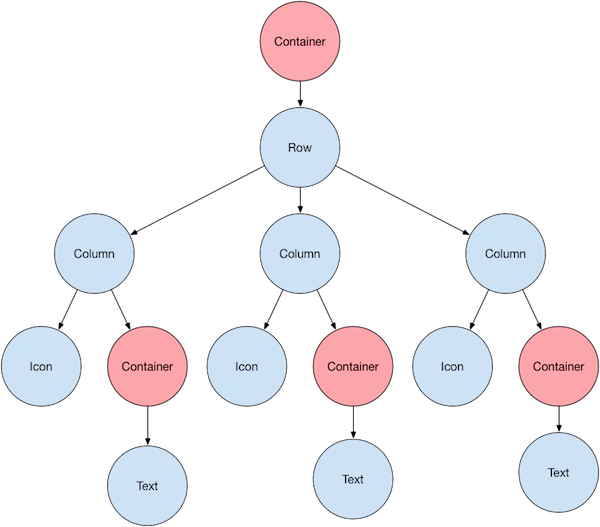
\includegraphics[height=7cm,keepaspectratio]{images/sample-flutter-layout.png} 
  \caption{Hierachie einer Menüleiste Quelle: Flutter Doku}
  \label{fig:flutter_layout_tree}
\end{figure}

Abbildung \ref{fig:flutter_layout_tree}

Um Seiten zu erstellen gibt es verschiedene Methoden. Oft muss man die Seiten komplett selbst aufbauen. Das heißt man fängt beim Startelement an. Dem sogennanten Scaffold. Dieser hat verschiedene Elemente. So gibt es AppBar man kann einen Footer hinzufügen und vorallem gibt es einen Body. Der kann dann ein Widget als Child hinzugefügt werden. Hier kann nun über verschiedene Widgets wieder neue Sachen hinzugefügt werden und so Stück für Stück ein Layout gebaut werden. 
Hierfür gibt es Grundsätzlich zwei verschiedene Arten von Widgets. 
1. Widgets die Helfen die Seite zu strukturieren und Layouts zu verfeinern und aufzubauen.
2. Widgets die Teil der Nutzeroberfläche sind und die unter Umständen noch weitere Childs zur ausgestaltung Besitzen, aber auf der Oberfläche angezeigt werden. So hat etwa ein TextButton noch ein Child Text wo dann der Text hinzugefügt wird, der im Button steht. Der Button ist allerdings ebenfalls ein Teil der UI. Anders als Container. Diese fügen eventuell eine Margin, also Abstand zu anderen Elementen hinzu oder ändern\TODO{Tun sie das wirklich?} unter Umständen auch mal den Hintergrund, sie sind allerdings keine Alleinstehenden Elemente und umgeben eigentlich nur das Child oder die Child Elemente.
\chapter{Entwicklung Hybrider Cross-Platform Application mit WebView und Flutter}

\subsection{Entwicklung einer Hybriden App mit wechsel zwischen Flutter und WebView}
In dem behandelten Beispiel wird Phoenix mit einer sogenannten Live Komponente behandelt. Hier gibt es eine Methode namens Live-redirect. Diese kann zwischen zwei Live komponenten hin und her schalten. Dadurch wird kein erneuter URL Aufruf ausgeführt, der dann von einem URL Request mitbekommen wird. Hier findet jedeglich eine AJAX Abfrage statt, die hier nicht abgefangen werden kann.
Zwei Mögliche Lösungen:
1. Website umbauen, sodass ein richtiger Redirect genutzt wird: Nachteil -> Geringere Performance im Browser
2. App so bauen, dass kompletter Live Bereich abgebildet wird: Nachteil -> Views die Nativ gar nicht gebaut werden sollten, müssen unter umständen gebaut werden, um Funktionalität zu gewährleisten.

Weiteres Problem war die Navigation. Da in diesem Fall zur besseren Performance immer die gleiche WebView wiederverwendet wurde, war es ein konstantes Springen zwischen einer WebView und nativen Teilen. Wenn man nun im WebViewBrowser die zurück Taste aufruft, wird innerhalb der WebView zurück gegangen. Hier kommt allerdings das Problem, dass wenn eine Flutter Page dazwischen geschaltet wurde, 
\chapter{Zusammenfassung und Auswertung}
\chapter{Fazit}


\vfill
\pagebreak

\appendix

% ----------------------------------------------------------------------------------------------------------
% Abkürzungsverzeichnis (optional, bitte nur wenn sinnvoll)
% ----------------------------------------------------------------------------------------------------------
%\listoftables
\addchap{Abkürzungsverzeichnis}
\begin{acronym}[KDE]
\acro{BA}[BA]{Bachelorarbeit}
\end{acronym}
\vfill
\pagebreak


% ----------------------------------------------------------------------------------------------------------
% Filter fuer Literatur und Quellen definieren
% ----------------------------------------------------------------------------------------------------------

\defbibheading{Literatur}{\addchap{Literaturverzeichnis}} 
\defbibheading{Quellen}{\addchap{Internetquellenverzeichnis}} 
  
\defbibfilter{Literatur}{\not\keyword{online}} 
\defbibfilter{Quellen}{\keyword{online}} 


% ----------------------------------------------------------------------------------------------------------
% Literatur
% ----------------------------------------------------------------------------------------------------------

\printbibliography[heading=Literatur,filter=Literatur] 
\vfill

\pagebreak


% ---------------------------------------------------------------------------------------------------------- 
% Internetquellen 
% ---------------------------------------------------------------------------------------------------------- 

\printbibliography[title = {Quellenverzeichnis}, heading=Quellen,filter=Quellen] 

\pagebreak 

% ----------------------------------------------------------------------------------------------------------
% Anhang
% ----------------------------------------------------------------------------------------------------------
\appendix


\chapter{Anhang}

% \input{inhalt/suppl}


\pagebreak


% % ----------------------------------------------------------------------------------------------------------
% % Eigenschtändigkeitserklaerung
% % ----------------------------------------------------------------------------------------------------------
\include{inhalt/erklaerung}



\end{document}